\documentclass{scrartcl}
\usepackage{german}
\usepackage[T1]{fontenc}
\usepackage[latin1]{inputenc}
\usepackage[german]{babel}

% zusätzliche mathematische Symbole, AMS=American Mathematical Society
\usepackage{amssymb}

% fürs Einbinden von Graphiken
\usepackage{graphicx}

% für Namen etc. in Kopf- oder Fußzeile
\usepackage{fancyhdr}

% erlaubt benutzerdefinierte Kopfzeilen
\pagestyle{fancy}

% Definition der Kopfzeile
\lhead{
\begin{tabular}{ll}
Fisnik Zeqiri & 4306430 \\
Felix  Karg   & 4342014
\end{tabular}
}
\chead{}
\rhead{\today{}}
\lfoot{}
\cfoot{Seite \thepage}
\rfoot{}

\begin{document}
\section*{Antworten zum �bungsblatt Nr. 12}

\section*{Aufgabe 1}
\begin{itemize}
    \item[a)] [ Bild 1 ] \\
        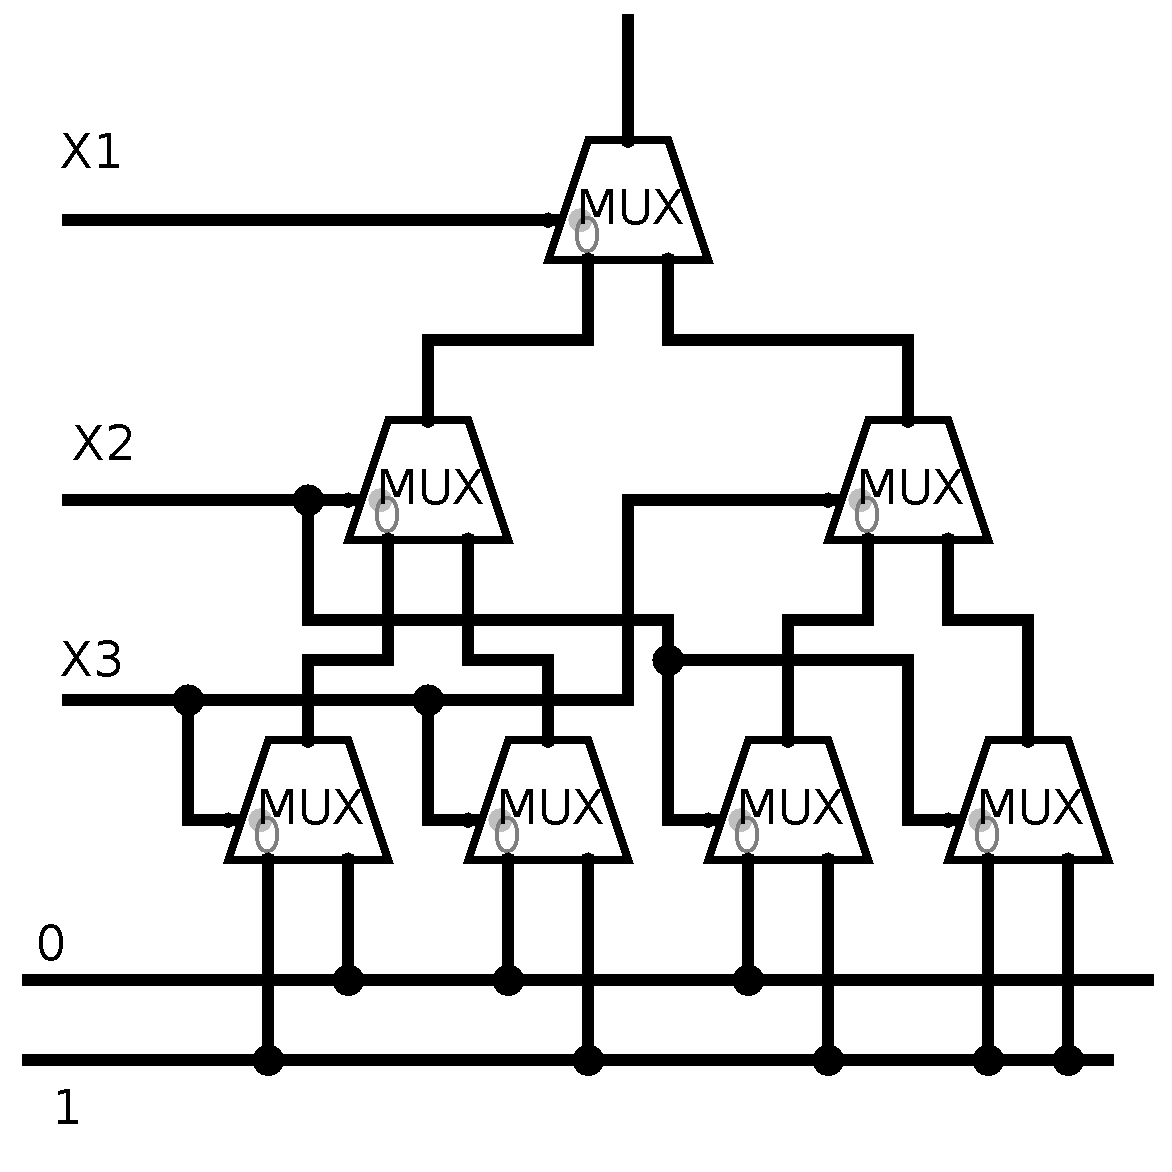
\includegraphics[width=11cm]{Muxer.png}
        \newpage
    \item[b)] Der in Abb. 2 dargestellte BDD ist weder geordnet
        (x2 kommt nach x3) noch reduziert (beim x2 ganz rechts ist
        es egal welche entscheidung man trifft). \\
        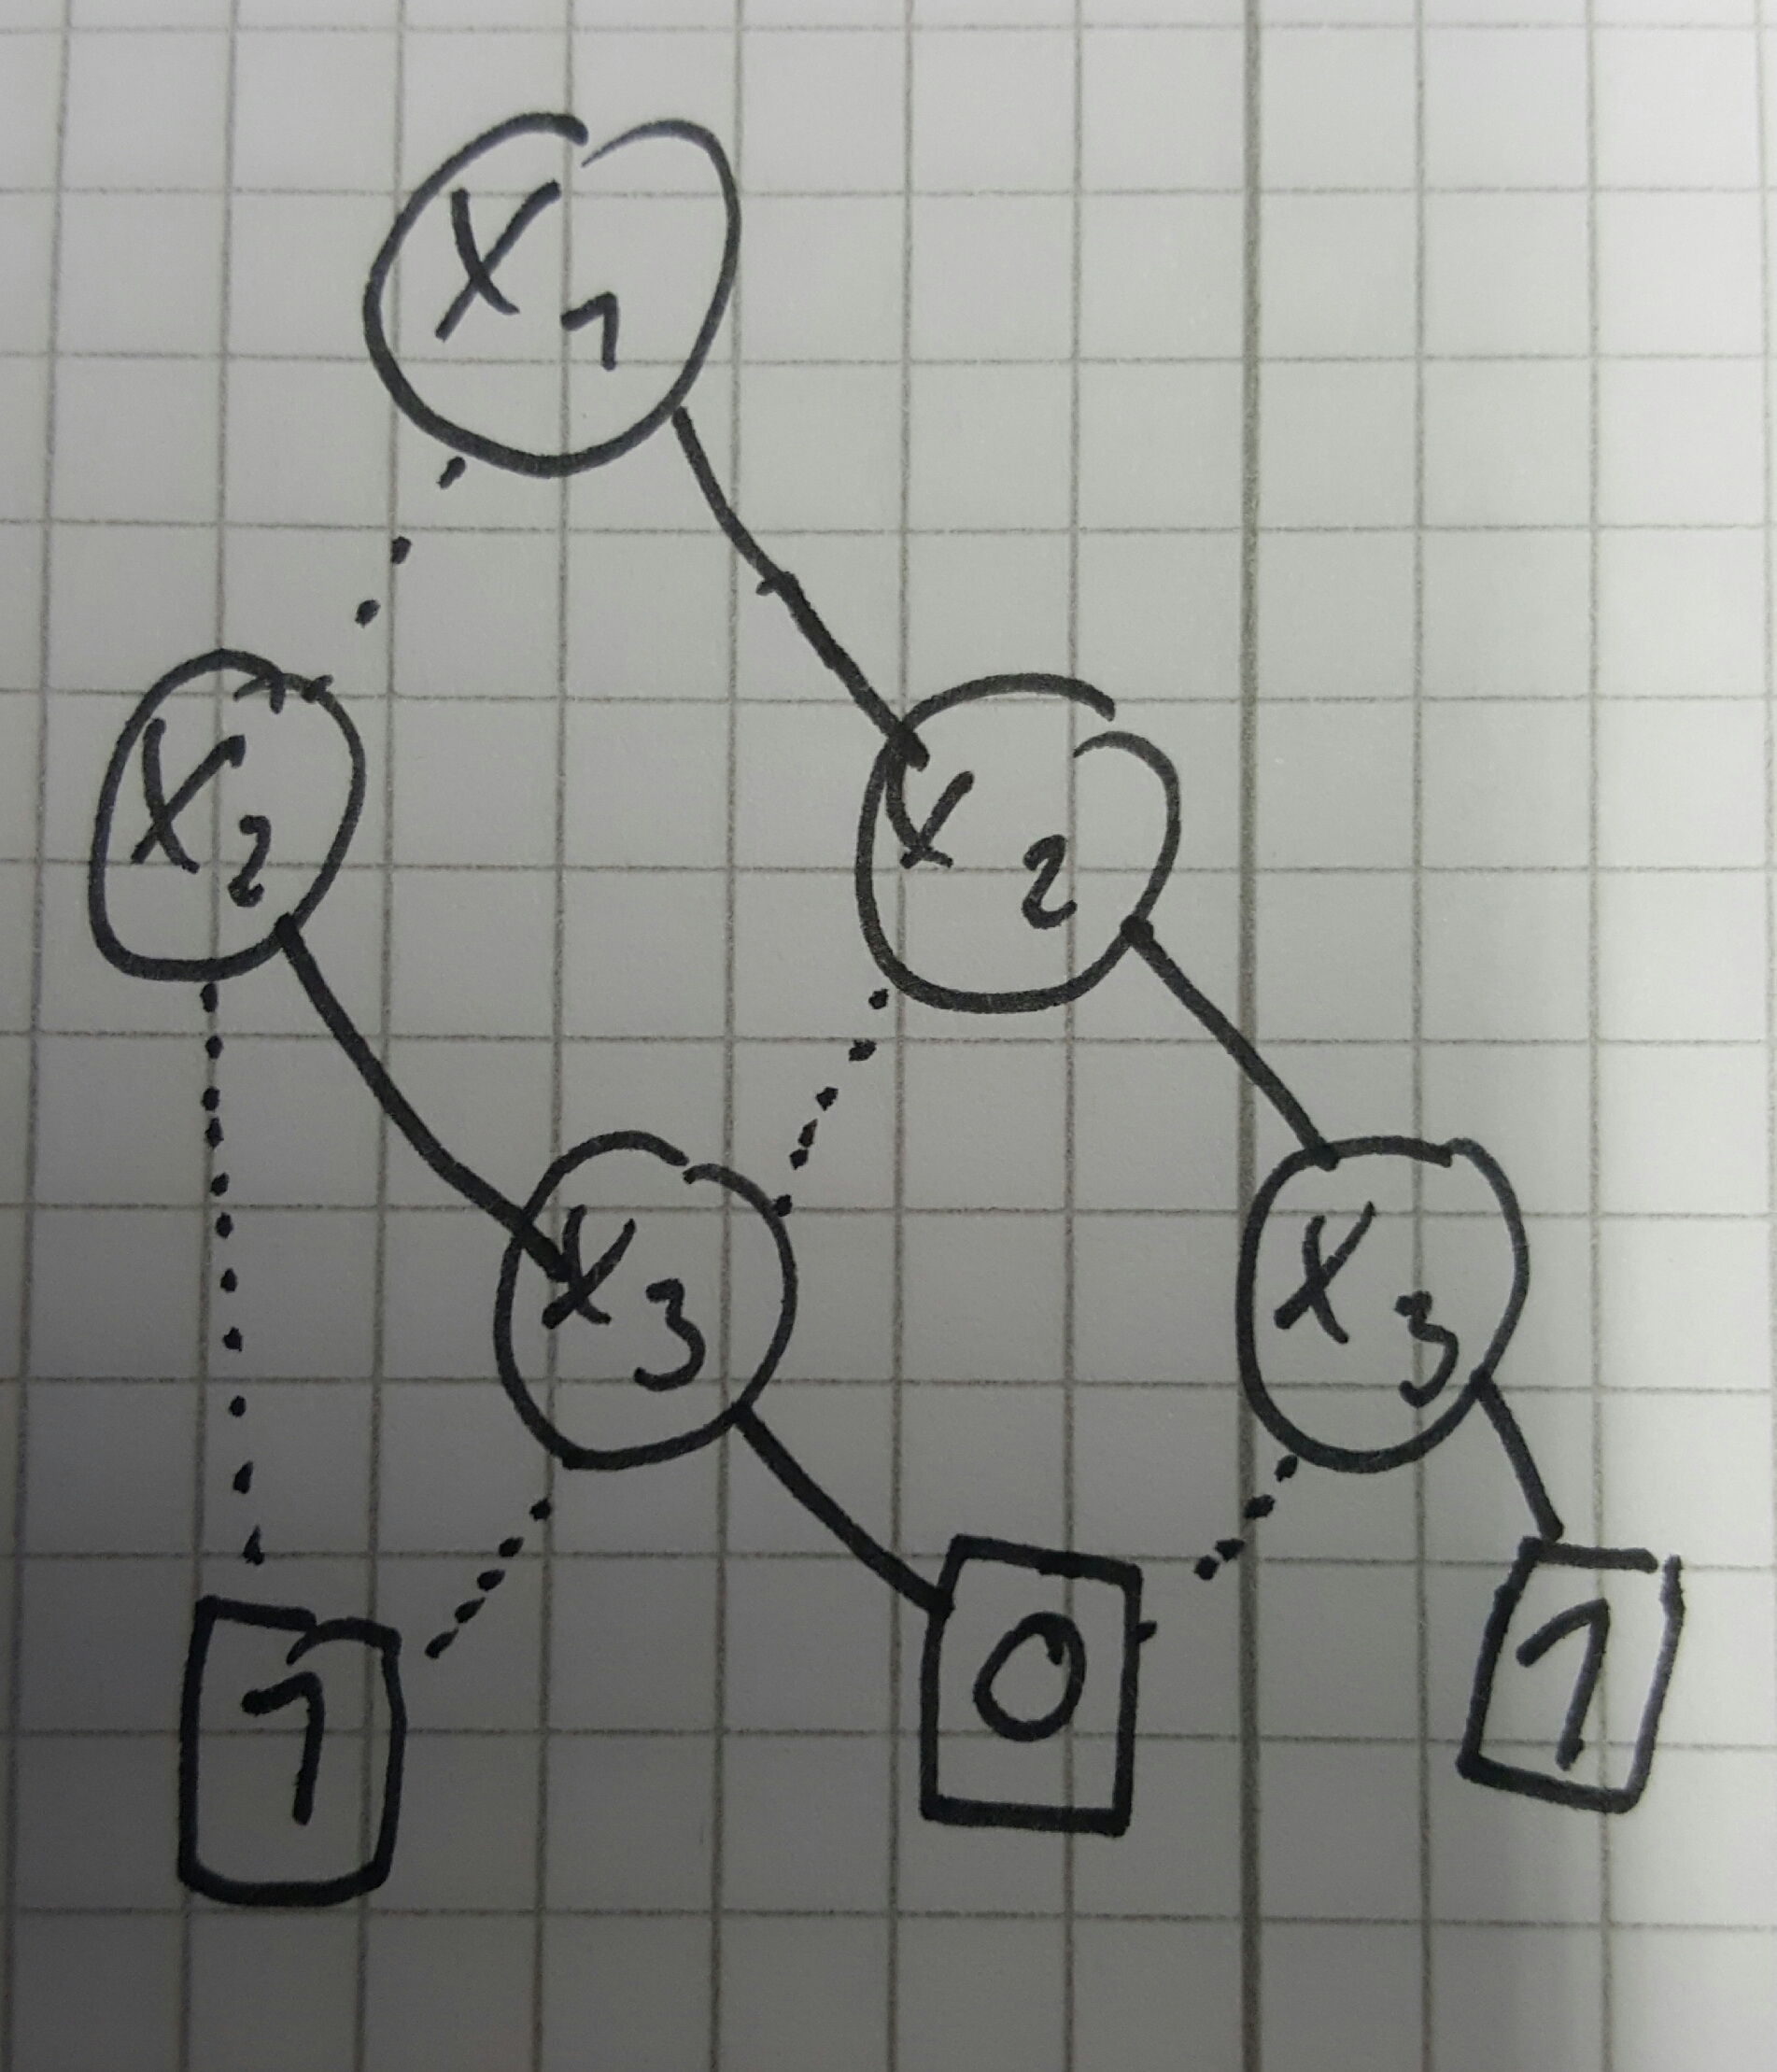
\includegraphics[width=11cm]{A1.jpg}
\end{itemize}

\newpage

\section*{Aufgabe 2}
\begin{itemize}
    \item[a)] [ Bild 2 ] \\
        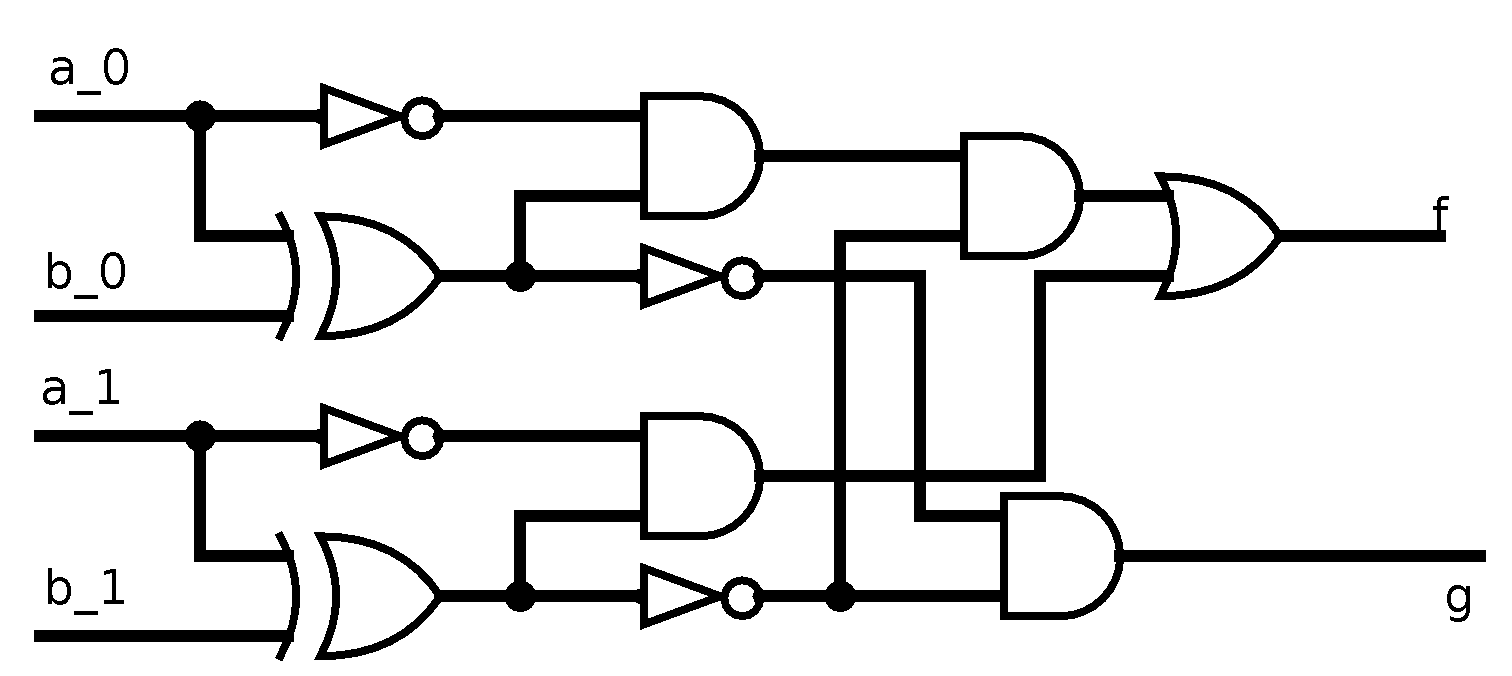
\includegraphics[width=14cm]{Komperator.png} \\
    \item[b)] [ Generieren von $f_{spez}$ und $g_{spez}$ ... ] \\
        % http://formal.cs.utah.edu:8080/pbl/BDD.php
        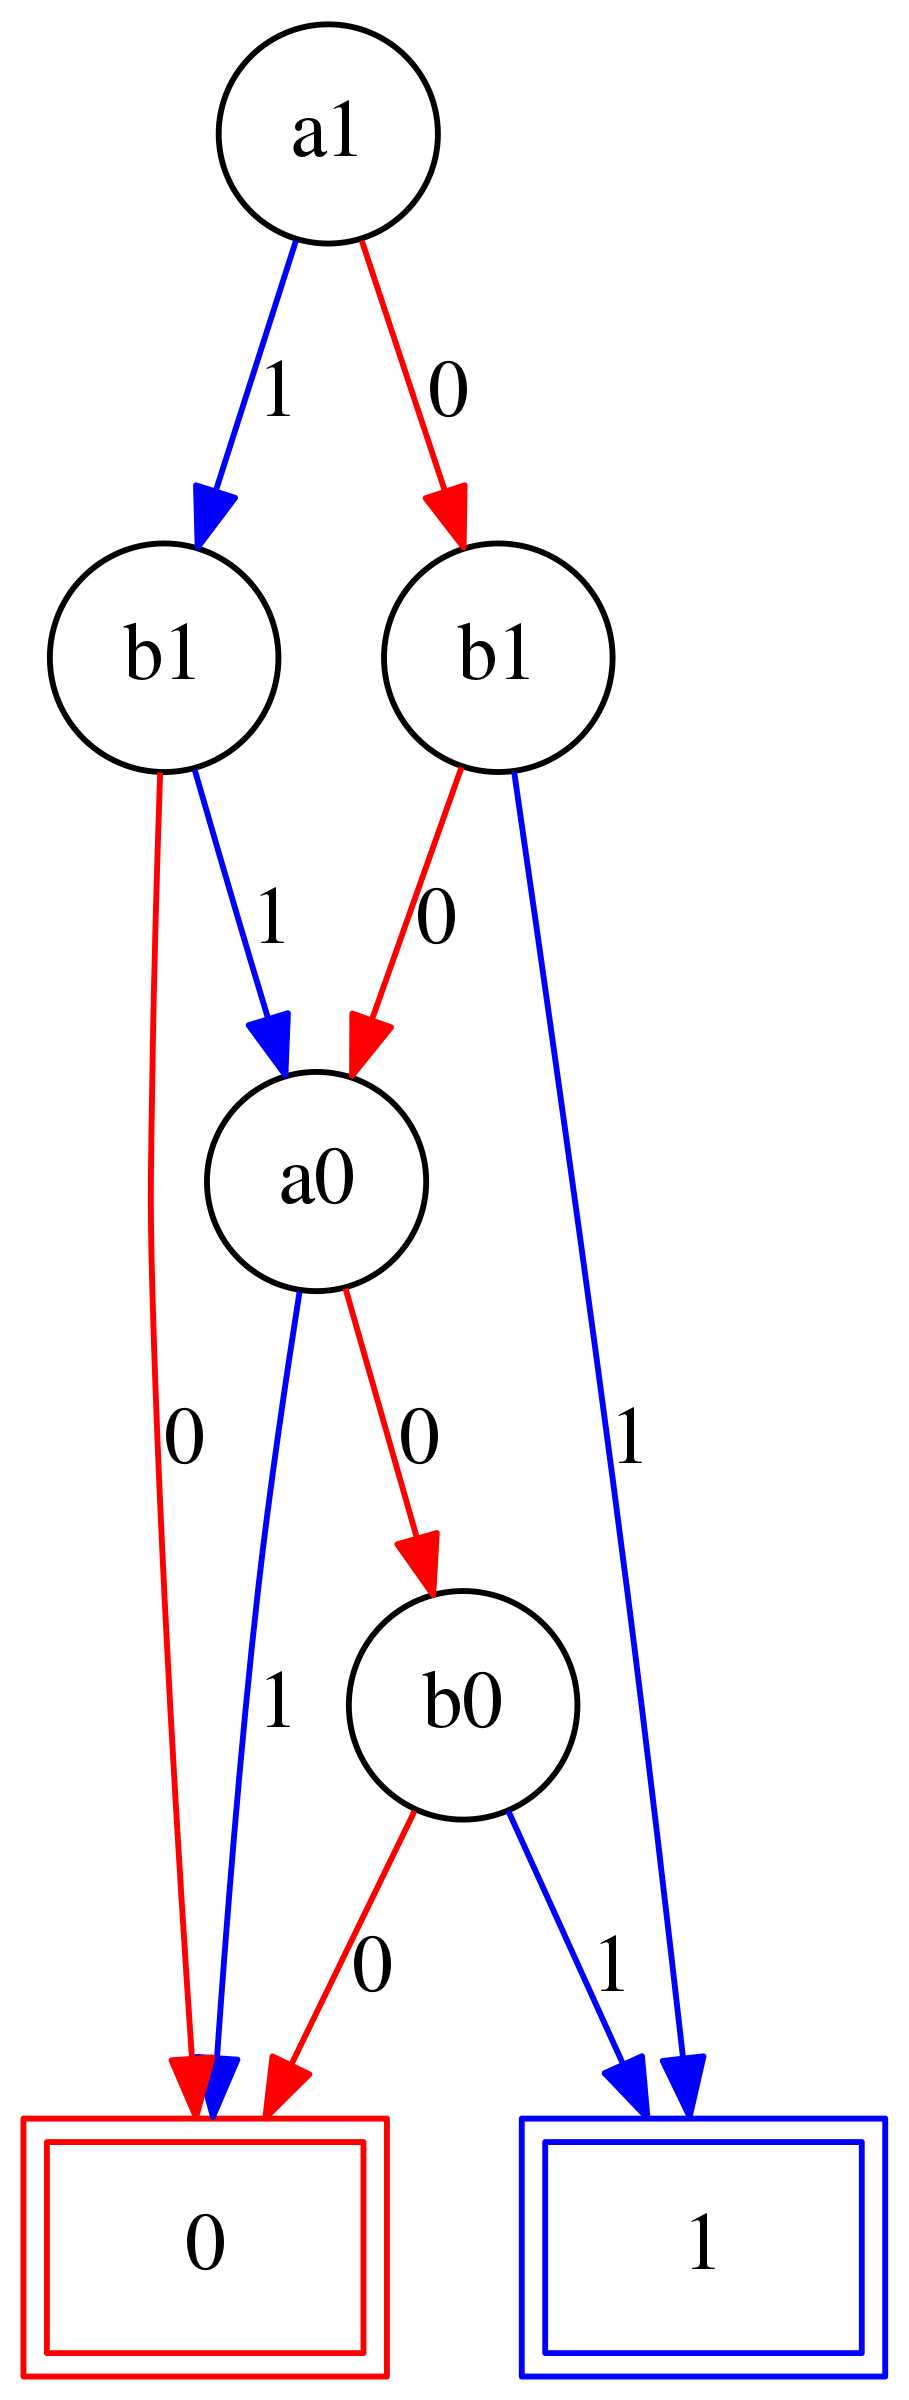
\includegraphics[width=4cm]{fspec.png}
        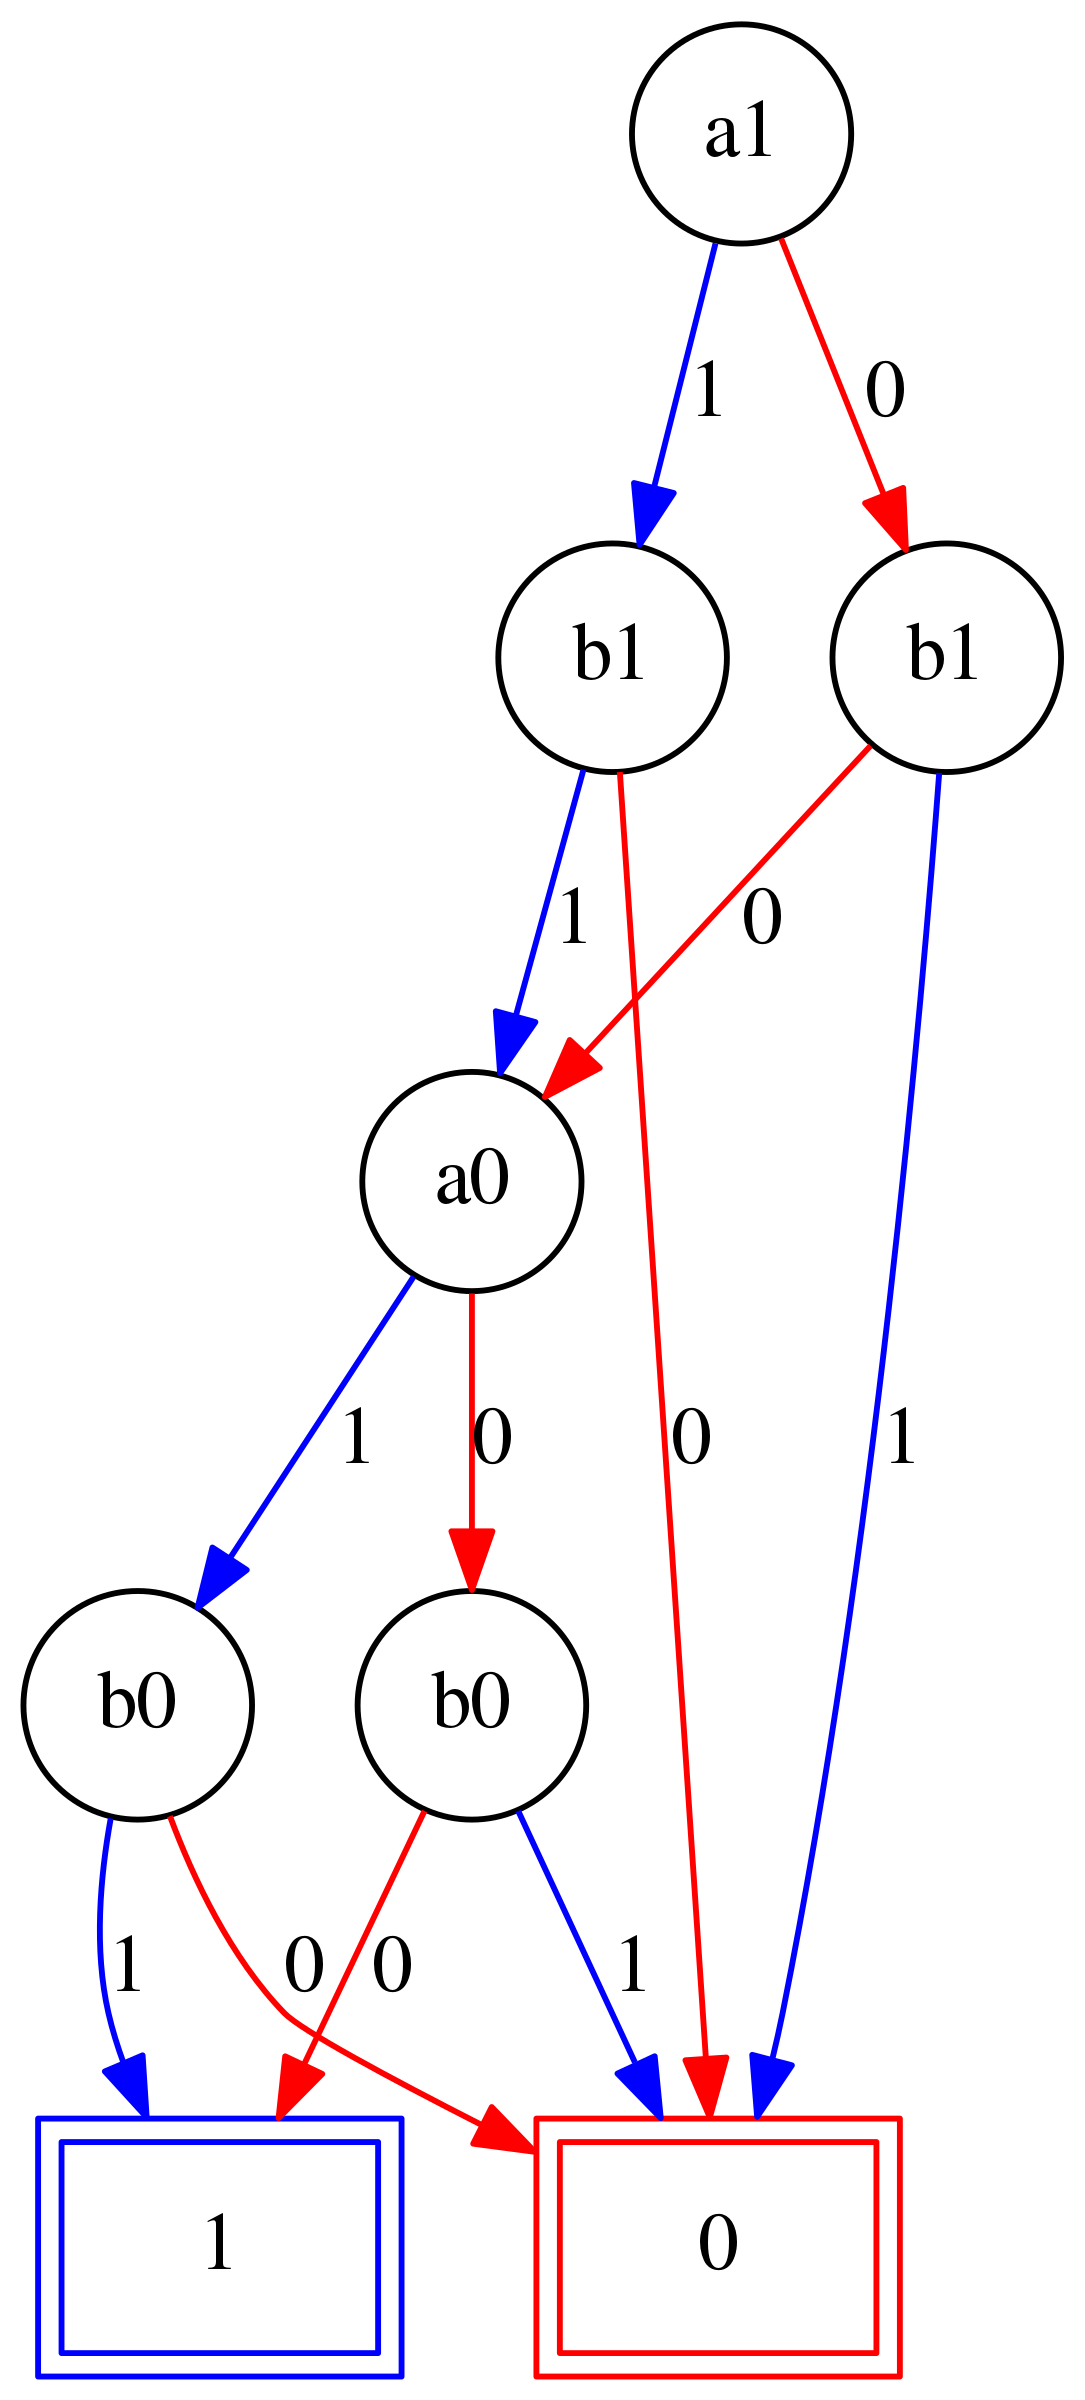
\includegraphics[width=5cm]{gspec.png} \\
        \newpage
        Ausformulieren von f und g: \\
        $ f = ((\sim a_0 \wedge (b_0 \oplus a_0)) \wedge \sim (a_1 \oplus b_1)) 
            \vee (\sim a_1 \wedge (a_1 \oplus b_1)) $ \\
        $ g = \sim(a_0 \oplus b_0) \wedge \sim(a_1 \oplus b_1) $ \\ \\
        Und daraus generierte geordnete reduzierte BDD's: \\
        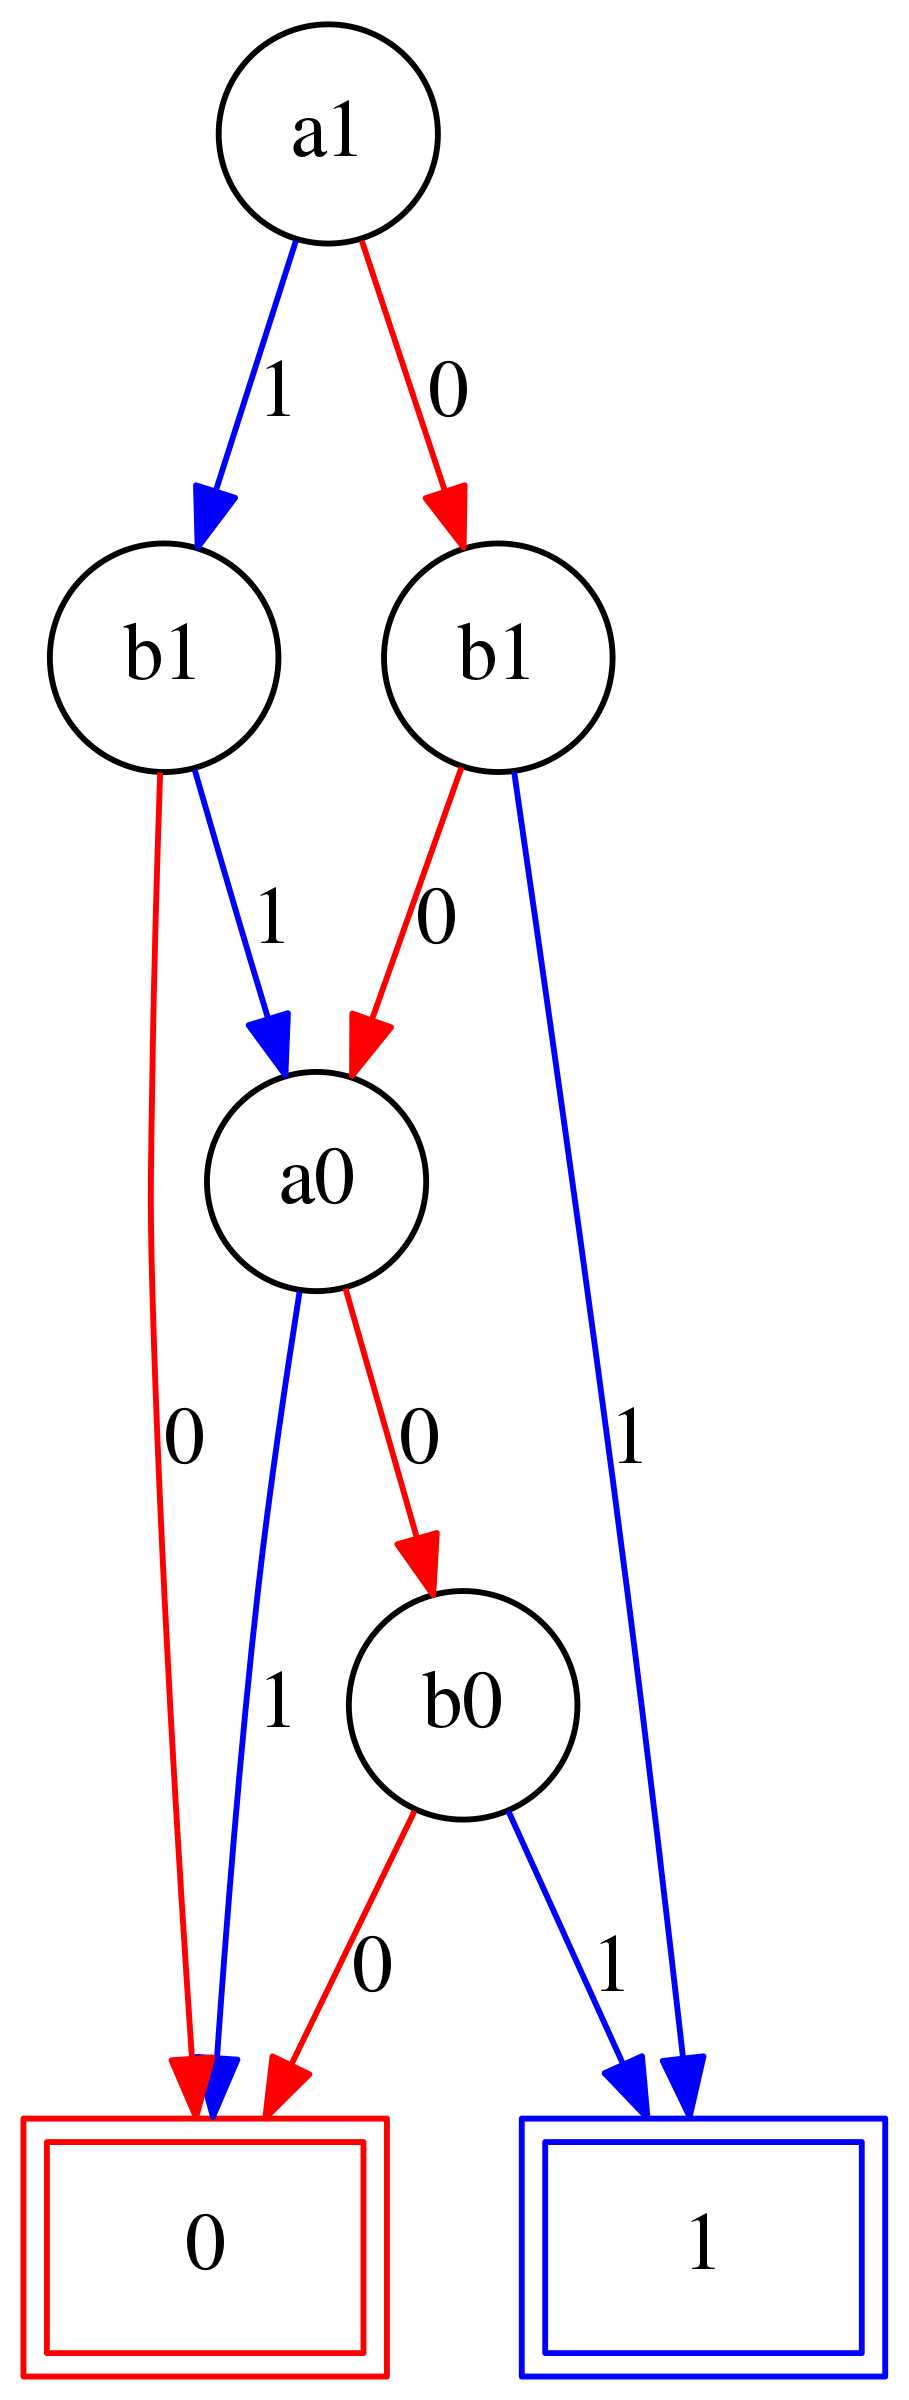
\includegraphics[width=4cm]{fspec.png}
        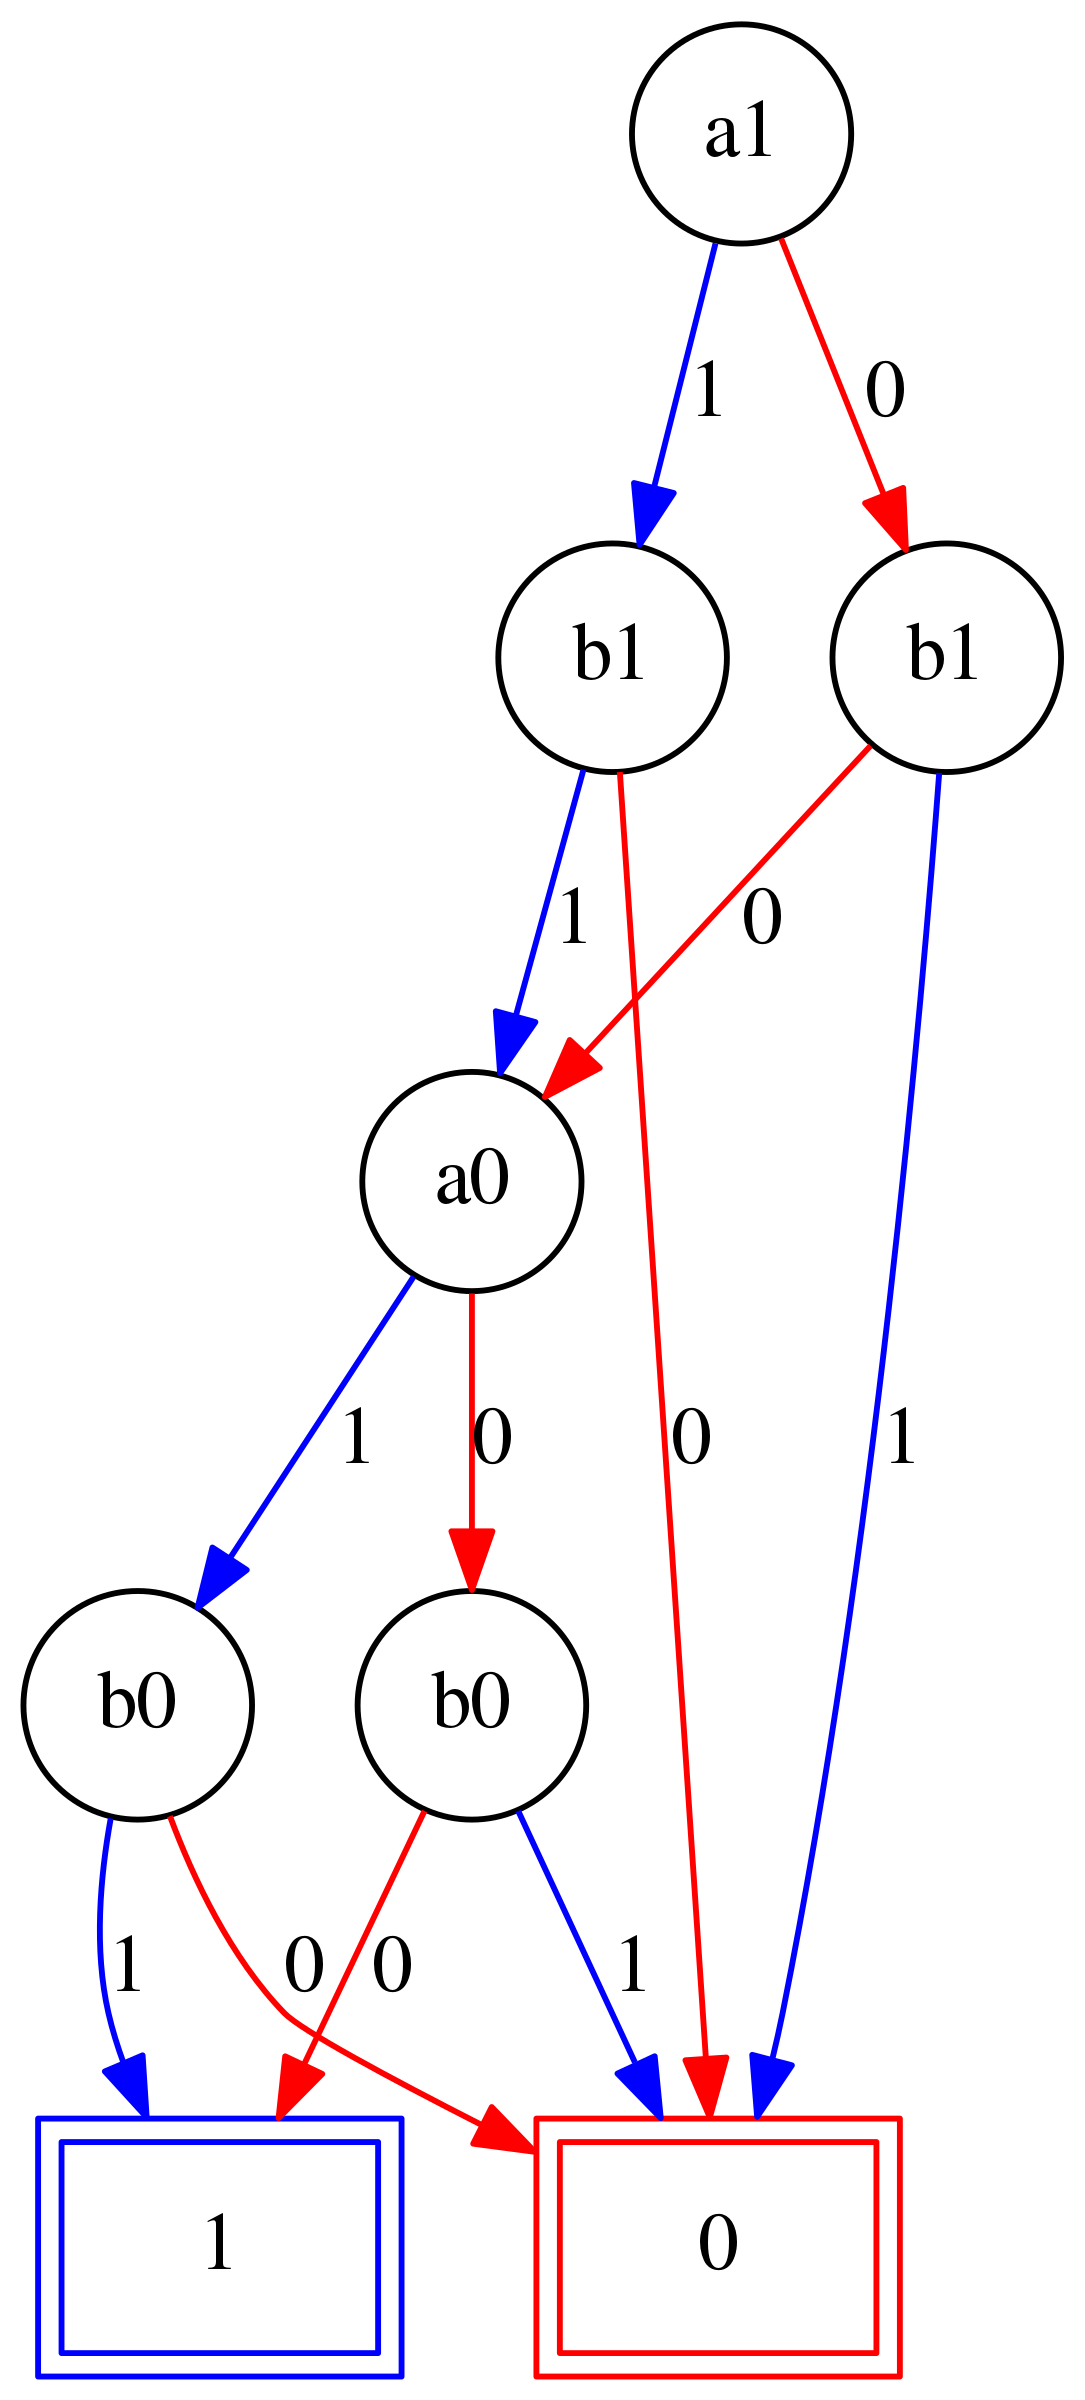
\includegraphics[width=5cm]{gspec.png} \\
    \item[c)] Feststellung: Beide gleich => Spezifikation wird erf�llt. \\
        \newpage
    \item[d)] $a_0$ und $b_0$ sind zus�tzlich die relativen Vorzeichenbits.
        Diese werden zuerst verglichen, da falls das vorzeichen $a$ 1 ist und
        das von b nicht, ist eindeutig a kleiner ist als b. \\
        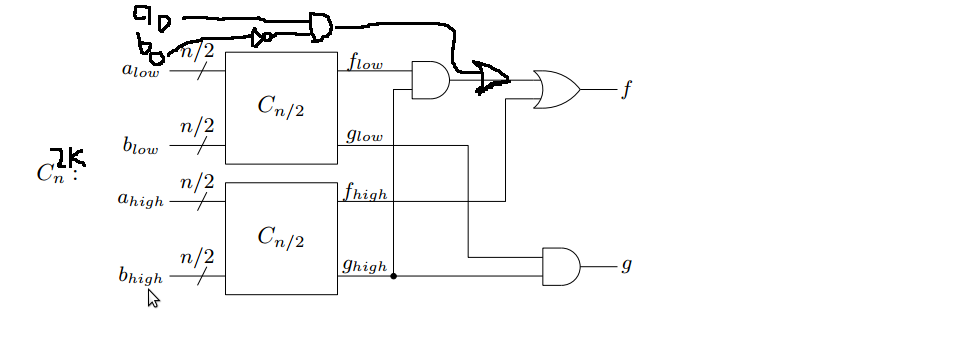
\includegraphics[width=12cm]{zweierkomplement.png}
\end{itemize}

\section*{Aufgabe 4}
\begin{itemize}
    \item[a)] [Folien:] Beschleunigung um $k - (k(k-1)/(m+k-1)) $ \\
        In unserem Fall: $k = 4, m_1 = 42, m_2 = 4711, m_3 = 27012017$ \\
        Also: $4 - 12/(m_i+3)$. $m_1 -> 3.7333, m_2 -> 3.9975, m_3 -> 3.9999 $, 
        Konvergiert also eindeutig gegen 4.
    \item[b)] NOPE.

\end{itemize}


\end{document}
